\documentclass[11pt,a4paper]{article}
\usepackage[utf8]{inputenc}
\usepackage[T1]{fontenc}
\usepackage[spanish,es-noshorthands]{babel}
\usepackage{lmodern}
\usepackage[margin=2.5cm]{geometry}
\usepackage{graphicx}
\usepackage{xcolor}
\usepackage{booktabs}
\usepackage{listings}
\usepackage{enumitem}
\usepackage[colorlinks=true,linkcolor=blue!50!black,urlcolor=blue!60!black]{hyperref}

\definecolor{codebg}{gray}{0.95}
\lstset{
  basicstyle=\ttfamily\small,
  backgroundcolor=\color{codebg},
  frame=single, rulecolor=\color{gray!50},
  keywordstyle=\color{blue!70!black}\bfseries,
  commentstyle=\color{gray}\itshape,
  stringstyle=\color{red!60!black},
  breaklines=true, columns=fullflexible,
  showstringspaces=false, upquote=true
}
\lstdefinelanguage{Dockerfile}{
  morekeywords={FROM,WORKDIR,COPY,RUN,EXPOSE,ENV,CMD},
  morecomment=[l]{\#}, morestring=[b]"
}

\begin{document}

\begin{titlepage}
  \centering
  {\large UNIVERSIDAD DEL VALLE\par}
  \vspace{0.2cm}
  {\normalsize Facultad de Ingeniería\par Escuela de Ingeniería de Sistemas y Computación\par}
  \vspace{0.4cm}
  {\normalsize MAESTRÍA EN COMPUTACIÓN PARA DESARROLLO DE APLICACIONES INTELIGENTES\par}
  \vspace{3cm}
  {\Huge\bfseries Taller 01\par}
  \vspace{0.4cm}
  {\LARGE Despliegue de Servicios de Red\par}
  \vspace{0.6cm}
  {\large Computación Distribuida y Frameworks para Desarrollo\\ de Aplicaciones Inteligentes\par}
  \vfill
  {\Large\bfseries CARLOS DAVID ROJAS LOZANO\par}
  \vspace{0.2cm}
  {\large Código: 202503497\par}
  \vspace{2cm}
  {\large Santiago de Cali, noviembre de 2026\par}
\end{titlepage}

\section{Resumen}
Se desplegó en una máquina virtual de AWS EC2 un servicio web que consulta y muestra el histórico de precios de la acción \textbf{GOOGL} desde el 2020-01-01. El servicio está escrito en Python con Flask y \texttt{yfinance}, se empaquetó como imagen Docker y se publicó en Docker Hub. Desde allí la VM lo descargó y lo ejecutó.

\begin{center}
\begin{tabular}{@{}ll@{}}
\toprule
\textbf{Elemento} & \textbf{Valor} \\
\midrule
Repositorio de código & \url{https://github.com/cadrojasl/taller01-despliegue-servicios} \\
Imagen Docker & \texttt{cadrojasl/stock-market:2.0} \\
Docker Hub & \url{https://hub.docker.com/r/cadrojasl/stock-market} \\
Nube & AWS EC2, región us-east-2 (Ohio), Ubuntu x86, t2.micro \\
URL pública & \url{http://ec2-3-145-6-64.us-east-2.compute.amazonaws.com} \\
\bottomrule
\end{tabular}
\end{center}

\section{Entregable 1: repositorio del código fuente y Dockerfile}

\textbf{Repositorio:} \url{https://github.com/cadrojasl/taller01-despliegue-servicios}

\begin{center}
\begin{tabular}{@{}lp{10cm}@{}}
\toprule
\textbf{Archivo} & \textbf{Función} \\
\midrule
\texttt{v2-flask/read\_value\_yf.py} & Descarga con \texttt{yfinance} los datos de un ticker entre una fecha inicial y hoy. \\
\texttt{v2-flask/app.py} & Expone esos datos como tabla HTML en la ruta \texttt{/} con Flask (puerto 5000). \\
\texttt{v2-flask/requirements.txt} & Dependencias: \texttt{yfinance}, \texttt{flask}. \\
\texttt{v2-flask/Dockerfile} & Construye la imagen \texttt{stock-market:2.0}. \\
\texttt{v1-script/} & Versión por consola (\texttt{stock-market:1.0}), ticker configurable con \texttt{-e STOCK=AMZN}. \\
\texttt{setup\_vm.sh} & Instala Docker en la VM y ejecuta el contenedor. \\
\bottomrule
\end{tabular}
\end{center}

\subsection*{Dockerfile}
\lstinputlisting[language=Dockerfile]{../v2-flask/Dockerfile}

\subsection*{app.py}
\lstinputlisting[language=Python]{../v2-flask/app.py}

\section{Entregable 2: servicio funcionando en la nube}
El servicio respondió desde la VM de AWS en la URL pública
\url{http://ec2-3-145-6-64.us-east-2.compute.amazonaws.com} y mostró la tabla de precios de GOOGL. Después de la prueba se terminó la instancia para no consumir créditos, así que la URL ya no responde. La evidencia es la siguiente captura.

\begin{figure}[h]
  \centering
  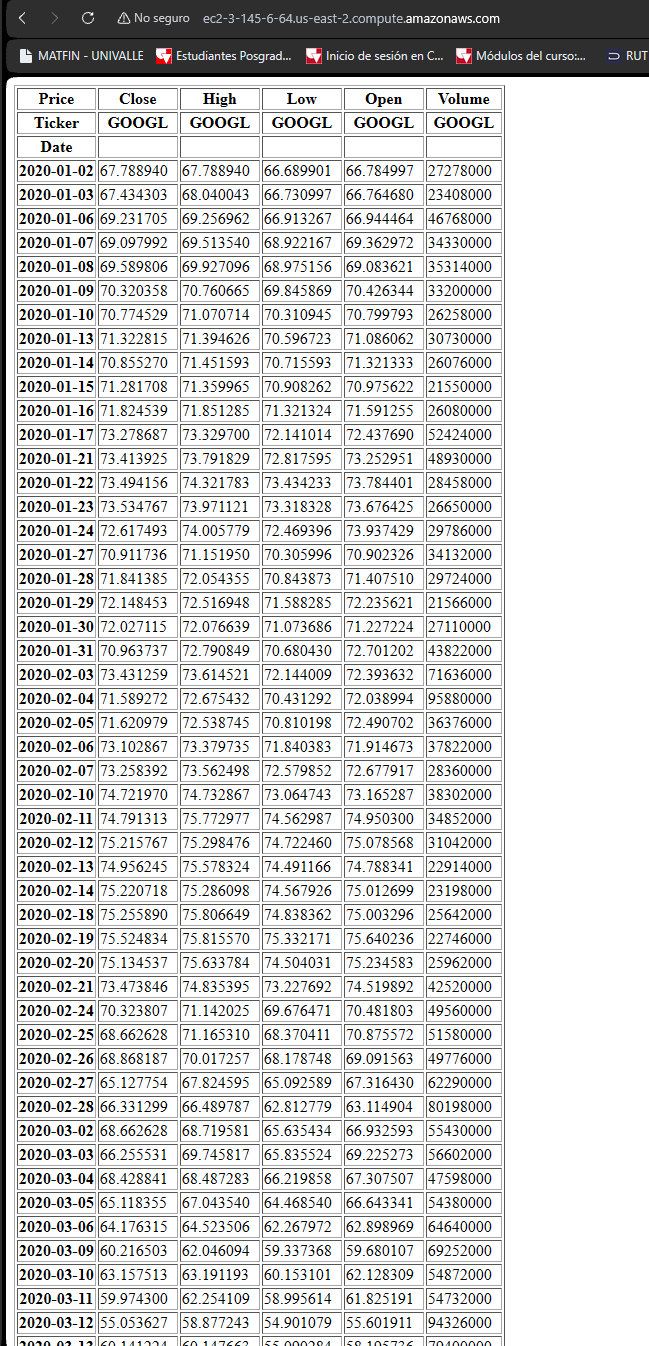
\includegraphics[height=0.62\textheight]{captura_aws.png}
  \caption{Servicio \texttt{stock-market} respondiendo desde AWS EC2.}
\end{figure}

\section{Pasos de despliegue}
\begin{enumerate}[leftmargin=*]
  \item \textbf{Construcción y prueba local:}
\begin{lstlisting}[language=bash]
docker image build -t stock-market:2.0 v2-flask
docker container run --rm -p 5000:5000 stock-market:2.0
\end{lstlisting}
  \item \textbf{Publicación en Docker Hub:}
\begin{lstlisting}[language=bash]
docker image tag stock-market:2.0 cadrojasl/stock-market:2.0
docker login
docker image push cadrojasl/stock-market:2.0
\end{lstlisting}
  \item \textbf{Creación de la instancia EC2} \texttt{demo\_docker}: Ubuntu x86, t2.micro, llave \texttt{demo\_docker.pem} y tráfico HTTP permitido en el Security Group.
  \item \textbf{Instalación de Docker en la VM} y permiso al usuario \texttt{ubuntu}:
\begin{lstlisting}[language=bash]
curl -fsSL https://get.docker.com | sudo sh
sudo usermod -aG docker ubuntu
\end{lstlisting}
  \item \textbf{Ejecución del contenedor:} el puerto 80 de la VM, abierto por el Security Group, se redirige al 5000 donde escucha Flask.
\begin{lstlisting}[language=bash]
sudo docker run -d --name stock-market -p 80:5000 cadrojasl/stock-market:2.0
\end{lstlisting}
  \item \textbf{Verificación} en el navegador con el Public IPv4 DNS y \textbf{terminación} de la instancia.
\end{enumerate}

\end{document}
